% !TEX encoding = UTF-8
% !TEX TS-program = pdflatex
% !TEX root = ../tesi.tex

%**************************************************************
\chapter{Resoconto dello stage}
\label{cap:resoconto}
%**************************************************************

\section{Descrizione del progetto}
Come descritto nella sezione \secref{sec:progetto} il progetto da portare a termine durante questo stage era un sistema di autenticazione personalizzato per \gls{zcsg}, che seguisse la tecnica del \gls{ssog}. \\

    \begin{figure}[h]
        \centering
        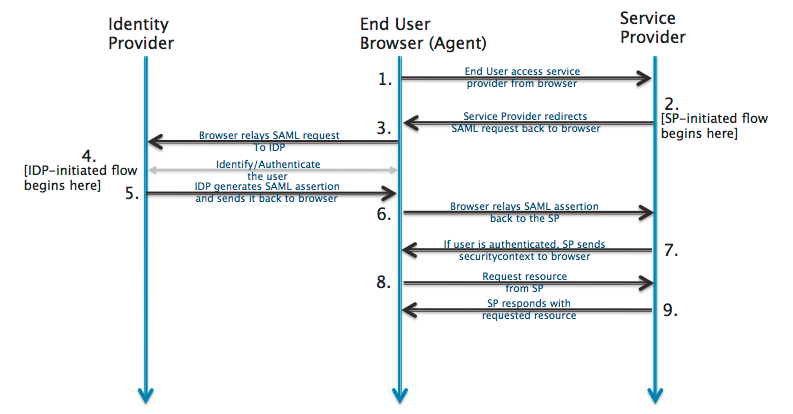
\includegraphics[width=1\textwidth]{immagini/sso_flow.png}
        \caption{\textit{Single Sign-On flow}}
        \textbf{Fonte}:
        \href{https://developer.okta.com/docs/concepts/saml/#federated-identity}{developer.okta.com}
        \label{fig: Single Sign-On flow}
    \end{figure}

Nel dettaglio, i miei compiti per questo progetto erano diversi. Per prima cosa dovevo trovare un protocollo di autenticazione che fosse adeguato alle esigenze dell'azienda e al problema da risolvere. Successivamente, dovevo passare alla progettazione di un sistema di autenticazione di base, che permettesse di effettuare il \textit{login} su \gls{zcsg} tramite \gls{okta}. Dal punto di vista pratico, all'utente era sufficiente cliccare su un'applicazione \textit{okta} presente nel pannello di controllo \textit{okta} oppure disponibile tramite estensione per \textit{browser}.

    \begin{figure}[h]
        \centering
        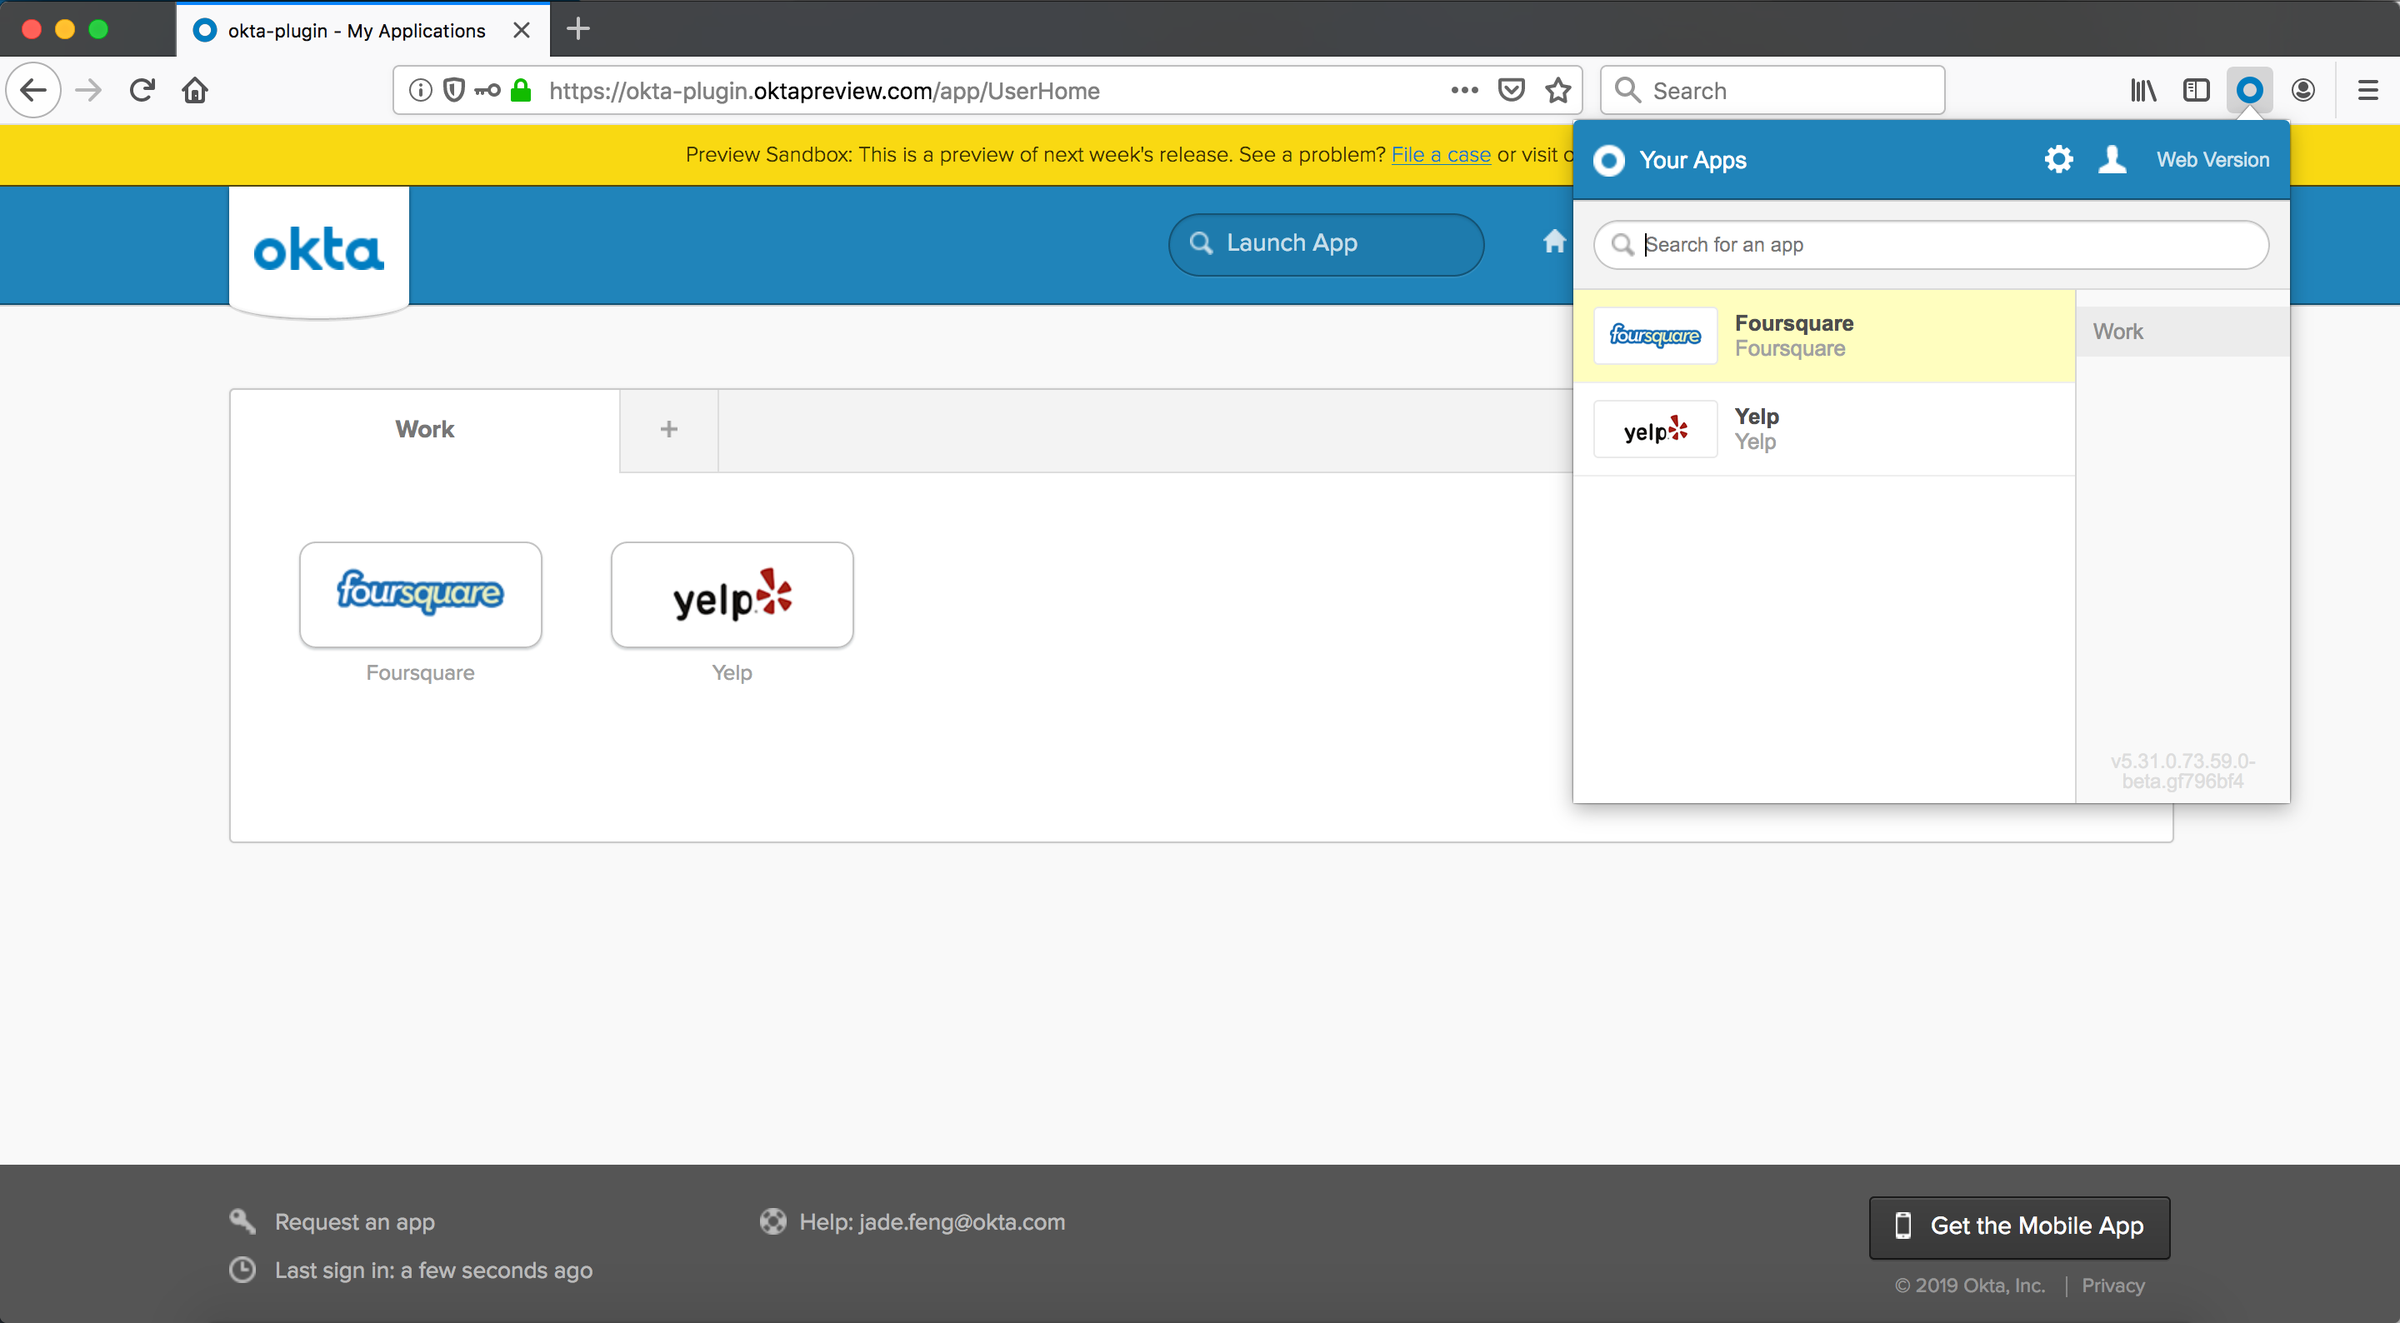
\includegraphics[width=1\textwidth]{immagini/okta_plugin.png}
        \caption{\textit{Okta plug-in}}
        \textbf{Fonte}:
        \href{https://addons.mozilla.org/en-US/firefox/addon/okta-browser-plugin/}{addons.mozilla.org}
        \label{fig: Okta plug-in}
    \end{figure}

Una volta effettuata l'autenticazione su \gls{okta} e premuto il pulsante relativo al \textit{login} per \gls{zcsg}, l'utente viene reindirizzato sulla \textit{webmail} di \gls{zcsg}.
Oltre a questa funzionalità era richiesto di creare un nuovo account su \gls{zcsg} qualóra l'utente \gls{okta} che sta tentando l'accesso non ne avesse ancora uno e, allo stesso tempo, fare una mappatura tra i gruppi a cui l'utente appartiene su \gls{okta} con le \gls{distlistg} e una \gls{cosg} di \gls{zcsg}. Per fare ciò, dovevo progettare un sistema apposito per stabilire come la mappatura dovesse avvenire dato che le informazioni tra i due sistemi potevano spesso risultare incompatibili. \\
L'architettura dell'intero sistema doveva essere un'estensione di \textbf{Zextras} che sfruttasse l'utilizzo di un \textit{handler http} ovvero un servizio che riceve delle richieste \textit{HTTP} nelle stesse modalità delle \gls{restg}. Questo \textit{handler} doveva gestire lo scambio di informazioni tra \gls{zcsg} e \gls{okta}, processarle e infine eseguire le operazioni già discusse.

\section{Pianificazione}
La prima pianificazione delle attività da svolgere è stata fatta da me, insieme al \textit{tutor}, prima dell'inizio dello stage per poter avere un'idea generale delle tempistiche necessarie al completamento degli obiettivi. Come descritto nella sezione \secref{sec:vincoli_tempo}, la pianificazione originaria ha subito delle leggere modifiche, causa necessità di più tempo da dedicare ad alcune attività. Inoltre, pur seguendo il piano di lavoro originale, la definizione di ciò che andava fatto ogni settimana veniva confermato una volta completato il lavoro che attualmente in corso.\\
Infatti dopo gli incontri formali fissati dal \textit{Project Manager} in cui dovevo mostrare i progressi tramite una \gls{demog}, vi erano spesso delle nuove richieste oppure delle modifiche da effettuare a ciò che avevo presentato. Per questo motivo, dopo ciascuno di questi incontri, mi fermavo per discutere con il \textit{team} quanto emerso e decidere come agire di conseguenza. Nella prima fase, descritta nel capitolo \secref{sec:att_analisi}, mi sono dedicato allo studio individuale dei protocolli e ho gestito il mio tempo autonomamente. Ogni giorno, durante il \textit{daily scrum}, aggiornavo il \textit{team} sui miei progressi e nel resto della giornata mi consultavo con loro in caso di necessità. Dopo questa prima attività era giunto il momento di creare la prima \textit{demo} che utilizzasse correttamente il protocollo scelto. Questa si è rivelata quella che ha consumato più tempo di quanto preventivato poiché, anche il \textit{team} non aveva mai fatto uso diretto di questo protocollo.\\
Tuttavia, una volta superato questo ostacolo, il lavoro è proseguito secondo il piano di lavoro originale con alcune accelerazioni nell'implementazioni di alcuni requisiti che si sono rivelati essere piuttosto semplici. Nella parte finale dello stage ho avuto inoltre la possibilità di eseguire delle attività fuori pianificazione, infatti ho eseguito alcune modifiche al prodotto successivamente al suo rilascio in ambiente di produzione.


\section{Analisi}
Come già discusso nella sezione \secref{sec:att_analisi}, l'attività di ricerca e analisi dei protocolli di autenticazione, è stata la prima attività svolta. Infatti, nei primi giorni di stage abbiamo discusso con il \textit{team} per stabilirne le modalità. Successivamente abbiamo individuato il primo requisito principale, ovvero l'autenticazione base di un utente su \gls{zcsg} tramite l'\gls{idpg} \gls{okta}. Il resto dei requisiti sono stati analizzati nel dettaglio dopo l'implementazione del primo, poiché ci serviva avere una base di partenza funzionante, al fine di capire cosa si potesse implementare e cosa invece non fosse fattibile. \\
Dopo aver capito le possibilità che avevamo, abbiamo stabilito che il sistema da progettare doveva essere modulare dal punto di vista degli \gls{idpg} supportati e, allo stesso tempo, dovevamo avere la possibilità di implementare dei servizi specifici per quanto riguarda l'integrazione delle configurazioni utente di \gls{zcsg} e \gls{okta}. Abbiamo dovuto prendere delle decisioni per quanto riguarda questo aspetto. Ad esempio l'associazione tra i gruppi a cui un utente \gls{okta} appartiene e la \gls{cosg} a cui il corrispettivo utente \gls{zcsg} appartiene poteva essere solo di tipo uno a uno. Per soddisfare un requisito di questo genere ho dovuto pensare ad una soluzione \textit{ad hoc} che richiedeva di avere in mano un sistema di base funzionante, capace di mettere in atto una comunicazione tra \gls{zcsg} e \gls{okta}. \\
I requisiti raccolti in seguito all'attività di analisi sono:
\begin{itemize}
    \setlength\itemsep{0em}
    \item \textbf{Obbligatori}: 14;
    \item \textbf{Desiderabili}: 1;
    \item \textbf{Opzionali}: 2;
\end{itemize}
 
Alcuni di questi sono illustrati nella seguente tabella:

\begin{center}
    \begin{table}[h]
    \begin{tabular}{| l | p{10cm} |} % you can change the dimension according to the spacing requirements 
        \hline
        \textbf{Identificativo} & \textbf{Descrizione} \\ \hline  
        R01 & Autenticare un utente non esistente su \gls{zcsg} tramite \gls{okta}, previa creazione dell'account\\ \hline
        R05 & Durante il processo di creazione di un nuovo utente su \gls{zcsg}, aggiungerlo alle giuste \gls{distlistg} a seconda dei gruppi a cui appartiene du \gls{okta}\\ \hline
        R08 & Durante la fase si autenticazione su \gls{zcsg} effettuato tramite \gls{okta}, aggiornare le \gls{distlistg}, se i gruppi a cui l'utente appartiene su \gls{okta} sono cambiati\\ \hline
        R11 & Configurazione del protocollo \gls{samlg} a livello di dominio\\ \hline
        R14 & Autenticazione a due fattori\\ \hline 
    \end{tabular}
    \caption{Tabella dei requisiti}
    \end{table}
\end{center}
\newpage

%**************************************************************
\section{Scelta del protocollo di autenticazione}
In seguito all'analisi condotta sui protocolli di autenticazione, accennata nella sezione \secref{sec:att_analisi}, sono emersi due protocolli di interesse, che ho proposto e discusso insieme al \textit{team}.
I due protocolli individuati erano \gls{samlg} e \gls{openidg}. Di seguito illustrerò i vantaggi e gli svantaggi di ciascuno.

\subsection{SAML}
    \subsubsection{Vantaggi}
    \begin{itemize}
        \item Fornisce meccanismi di sicurezza nel momento in cui la connessione \textit{HTTPS} non è disponibile o potrebbe essere compromessa;
        \item Si tratta di uno dei protocolli più utilizzati e affermati sul mercato;
        \item Se implementato correttamente è molto affidabile e sicuro;
        \item Il meccanismo chiamato \textit{federated identity} permette di ridurre i costi per la gestione delle identità degli utenti che hanno accesso a più organizzazioni.
    \end{itemize}
    \subsubsection{Svantaggi}\label{sec:saml_svantaggi}
    \begin{itemize}
        \item Nell'implementazione di alcuni casi d'uso è necessario effettuare dei reindirizzamenti \textit{HTTP}, che conviene eseguire con una richiesta \textit{POST}. Il problema risiede nel fatto che per poterla fare in automatico è necessario scrivere del codice in più con un altro linguaggio;
        \item Per il problema evidenziato al punto precedente, non è facile implementare questo protocollo su applicazioni native per dispositivi mobili;
        \item Essendo un protocollo basato su \gls{xmlg}, soffre di una tipologia di attacchi chiamati \textit{XML Signature Wrapping}, che potrebbero modificare i documenti \gls{xmlg} scambiati fra le parti del protocollo;
        \item L'\gls{xmlschemag} del protocollo è particolarmente complesso.
    \end{itemize}

\subsection{OpenID}
    \subsubsection{Vantaggi}
    \begin{itemize}
        \setlength\itemsep{0em}
        \item I \textit{JSON Web Token (JWT)} utilizzati per rappresentare le informazioni dell'autenticazione sono in un formato portabile e moderno e supportano diversi algoritmi di crittografia;
        \item Essendo basato su un altro protocollo chiamato \gls{oauthg}, il quale funziona su applicazioni mobile native, permette di essere implementato su di esse;
        \item Essendo basato su un protocollo di autorizzazione, citato al punto precedente, con \gls{openidg} si ha un singolo protocollo per autenticazione e autorizzazione;
        \item Facile da implementare.
    \end{itemize}
    \subsubsection{Svantaggi}
    \begin{itemize}
        \setlength\itemsep{0em}
        \item Al momento dell'analisi effettuata risultava essere una soluzione poco comune sul mercato, da ciò ne deriva la mancanza di \textit{best practice};
        \item \textit{HTTPS} è l'unico livello di criptazione e sicurezza tra il \textit{client} e l'\gls{idpg}.
    \end{itemize}

\subsection{Motivazioni della scelta}
Dopo una discussione con il \textit{team} di sviluppo e il \textit{Project Manager}, abbiamo stabilito di utilizzare il protocollo \gls{samlg}. Le ragioni che ci hanno portato a sceglierlo sono le seguenti:
\begin{itemize}
    \item Essendo il protocollo molto diffuso, vi erano \textit{best practice} note e una comunità di sviluppatori più esperta;
    \item \gls{okta} supporta questo protocollo facilitando la comunicazione con un servizio personalizzato che implementa \gls{samlg};
    \item Disponibilità di una libreria scritta in \textit{Java}, il linguaggio utilizzato in azienda, già affermata e utilizzata in altre applicazioni che implementa le funzionalità base del protocollo. Tale libreria è \gls{opensg}, di fondamentale importanza visto la filosofia aziendale;
    \item Non vi era necessità di portare questo sistema di autenticazione su dispositivi mobili ma, nel caso in futuro ci fosse la necessità di farlo, ci sarebbero delle soluzioni valide per risolvere il problema descritto nella sezione \secref{sec:saml_svantaggi}.
\end{itemize}

\subsection{Il protocollo SAML}
Il protocollo \gls{samlg} coinvolge generalmente tre attori:
\begin{itemize}
    \item \textit{\textbf{Service provider}}: è l'entità che fornisce il servizio all'utente, solitamente un sito \textit{web} o una risorsa disponibile su di esso. In questo progetto è la \textit{webmail} di \gls{zcsg};
    \item \textit{\textbf{User-agent}}: è un software permette la fruizioni del contenuto ad un utente. Di solito un \textit{web browser} che renderizza i contenuti delle pagine \textit{web};
    \item \textit{\textbf{Identity Provider}}: è l'autorità che certifica l'identità di un utente. In questo progetto questo ruolo è assunto da \gls{okta}.
\end{itemize}
Un esempio di come queste tre parti interagiscono è illustrato nella figura \secref{fig: Single Sign-On flow}.
\gls{samlg} è costituito da diversi componenti che possono essere combinati tra di loro in diversi modi, a seconda del caso d'uso richiesto dal problema da risolvere. Le principali funzioni di questi componenti sono autenticazione, gestione dell'identità e autorizzazione tra organizzazioni che abbiano stabilito un rapporto di fiducia. I principali "concetti" del protocollo sono i seguenti:
\begin{itemize}
    \item \textit{\textbf{Assertion}}: è un documento in formato \gls{xmlg} che contiene le informazioni sull'autenticazione e/o autorizzazione di un utente. Tale documento è solitamente generato dall'\gls{idpg} e inviato al \gls{spg};
    \item \textit{\textbf{Protocols}}: sono dei meccanismi per fare in modo che vengano ritornate delle opportune risposte \textbf{SAML} a determinate richieste \textbf{SAML};
    \item \textit{\textbf{Bindings}}: definiscono il metodo di comunicazione a basso livello utilizzato dai partecipanti del protocollo. Per esempio permettono di specificare la comunicazione avviene tramite richieste \textit{HTTP} o \textit{SOAP};
    \item \textit{\textbf{Profiles}}: i profili definiscono una particolare configurazione di \textit{assertion}, \textit{protocols} e \textit{bindings} che serve per soddisfare un caso d'uso specifico;
    \item \textit{\textbf{Metadata}}: è un documento \gls{xmlg} che serve per condividere delle configurazioni tra le parti. Per esempio il metodo di crittografia delle asserzioni o di un insieme di attributi;
    \item \textit{\textbf{Authentication Context}}: è un meccanismo, definito da un \gls{xmlschemag}, che serve per descrivere la tipologia di autenticazione impiegata dall'utente quando si autentica con l'\gls{idpg}.
\end{itemize}

    \begin{figure}[h]
        \centering
        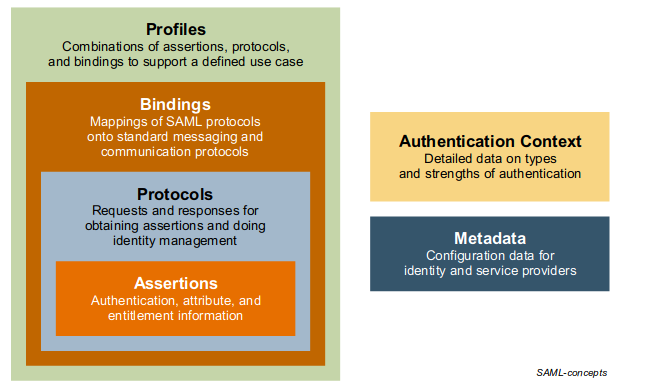
\includegraphics[width=0.95\textwidth]{immagini/SAMLCore.png}
        \caption{\textit{SAML Core concepts}}
        \textbf{Fonte}:
        \href{https://www.oasis-open.org/committees/download.php/27819/sstc-saml-tech-overview-2.0-cd-02.pdf}{oasis-open.org}
        \label{fig: SAML core}
    \end{figure}

\section{Progettazione}
%Progettazione della soluzione proposta per l'implementazione del sistema di autenticazione
\subsection{Configurazione applicazione Okta}
Un'applicazione \gls{okta} è un servizio basato sullo scambio di informazioni tramite \gls{restg} tra \gls{okta} e un'altro servizio \textit{web}. Sapendo che \gls{okta} supportava il protocollo \gls{samlg} e che in azienda erano state già create altre applicazioni \gls{okta} per integrazioni con gli strumenti utilizzati internamente, abbiamo stabilito che la cosa migliore da fare per comunicare con l'\gls{idpg} fosse quella di creare una \textit{SAML application} che avesse come \gls{endpointg} l'indirizzo dell'\textit{handler HTTP} descritto nella sezione successiva.
Di seguito un esempio di configurazione della \textit{okta application} con gli \gls{endpointg} dell'\textit{handler}.

    \begin{figure}[h]
        \centering
        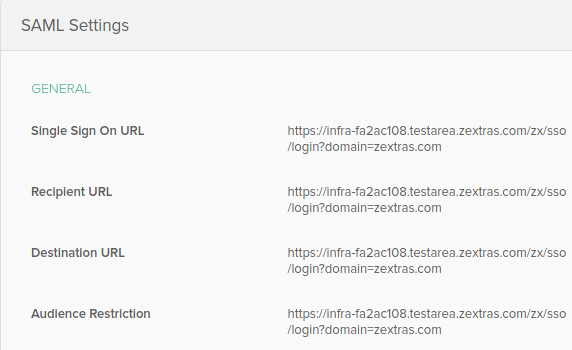
\includegraphics[width=1\textwidth]{immagini/endpoints.png}
        \caption{\textit{SAML endpoints}}
        %\textbf{Fonte}:
        %\href{https://www.oasis-open.org/committees/download.php/27819/sstc-saml-tech-overview-2.0-cd-02.pdf}{oasis-open.org}
        \label{fig: SAML endpoints}
    \end{figure}
Essendo questa un'applicazione specifica per \gls{samlg}, era possibile specificare quali attributi dell'utente inviare all'\textit{handler} (per esempio l'anagrafica e i gruppi a cui appartiene su \gls{okta}) per avere la possibilità non solo di autenticarlo, ma anche di creare il nuovo \textit{account} su \gls{zcsg} come già speficificato nella sezione \secref{sec:progetto}. Tali informazioni vengono inviate all'\textit{handler} tramite una \gls{samlass}. Di seguito un esempio di configurazione:
\newpage
    \begin{figure}[h]
        \centering
        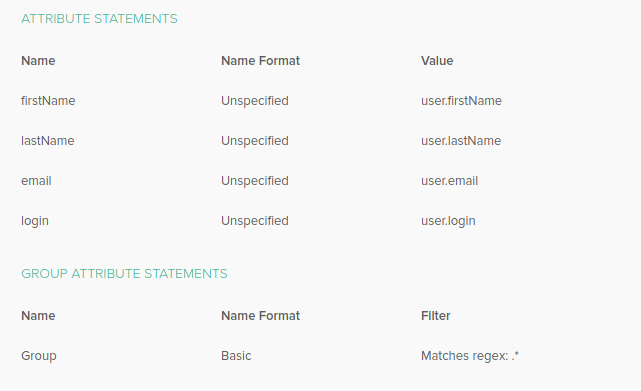
\includegraphics[width=1\textwidth]{immagini/saml_attributes.png}
        \caption{Attributi \textit{SAML}}
        %\textbf{Fonte}:
        %\href{https://www.oasis-open.org/committees/download.php/27819/sstc-saml-tech-overview-2.0-cd-02.pdf}{oasis-open.org}
        \label{fig: Attributi SAML}
    \end{figure}

\subsection{Progettazione handler HTTP}
I servizi \textit{web} di \textbf{Zextras} sono gestiti tramite degli \textit{handler HTTP}, ovvero delle classi \textit{Java} che restano in ascolto su uno o più \gls{endpointg} tramite i quali ricevono dei dati. Questi vengono elaborati e viene generata una risposta che può ridursi ad un'azione eseguita, un messaggio di ritorno oppure un reindirizzamento ad una certa pagina \textit{web}. In particolare l'\textit{handler} che gestiva tutte le operazioni che il mio sistema doveva svolgere, doveva ricevere una \textit{SAML Response}, cioè un documento \gls{xmlg} con una \gls{samlass} al suo interno. L'asserzione conteneva i dati dell'utente con i quali era possibile:
\begin{itemize}
    \setlength\itemsep{0em}
    \item Autenticare l'utente;
    \item Creare il nuovo account su \gls{zcsg} al primo tentativo di \textit{login};
    \item Assegnare l'utente alla giusta \gls{cosg} e alle \gls{distlistg}.
\end{itemize}
\subsection{Sistema di mappatura dei gruppi Okta}
Una volta giunti i dati all'\textit{handler HTTP} era necessario prendere una decisione su come mappare i gruppi a cui l'utente apparteva su \gls{okta} con una sola \gls{cosg} e allo stesso tempo più \gls{distlistg} di \gls{zcsg}. Purtroppo ciò non era possibile eseguire questa operazione in automatico poiché se un utente apparteneva ad un gruppo chiamato A su \gls{okta}, il sistema avrebbe dovuto inserire l'utente in una \gls{cosg} chiamata A. Il problema è analogo per le \gls{distlistg}, in quanto un gruppo di nome A doveva essere mappato sulla lista denominata "A@dominio", ma l'esistenza di tale dominio su \gls{zcsg} non era garantito. Per i motivi sopra elencati, tentare una mappatura automatica avrebbe portato ad errori e comportamenti inattesi. \\
Ho investito un po' di tempo per cercare una soluzione e ho proposto di dare la possibilità all'amministratore di \gls{okta} e \gls{zcsg} di configurare manualmente le associazioni desiderate tramite un \textit{file} in formato \gls{jsong}. Nel caso della \gls{cosg}, la quale è unica per ciascun utente, era possibile effettuare un'associazione uno a uno tra gruppo di \gls{okta} e \gls{cosg}, a patto che questa esista su \gls{zcsg}. In caso contrario il sistema ignora l'associazione in fase di mappatura. Per quanto riguarda le \gls{distlistg}, era possibile associare un gruppo \gls{okta} con una lista di \gls{distlistg} presenti su \gls{zcsg}.
Una volta discussa e approvata dal \textit{team} e dal \textit{Project Manager} ho messo in atto quanto descritto. Di seguito un esempio di mappatura per la \gls{cosg} e le \gls{distlistg}.

    \begin{figure}[h]
        \centering
        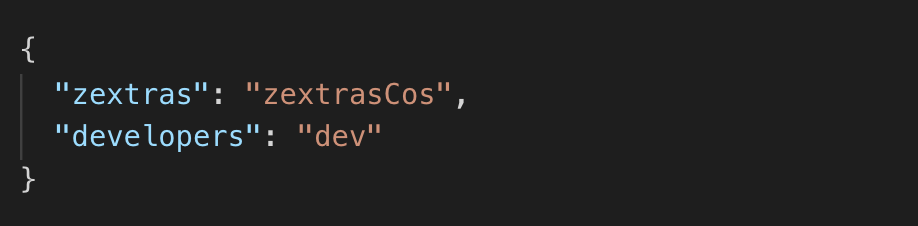
\includegraphics[width=1\textwidth]{immagini/cosMapping.png}
        \caption{Mappatura classe di servizio}
        %\textbf{Fonte}:
        %\href{https://www.oasis-open.org/committees/download.php/27819/sstc-saml-tech-overview-2.0-cd-02.pdf}{oasis-open.org}
        \label{fig: Mappatura classe di servizio}
    \end{figure}
    
     \begin{figure}[h]
        \centering
        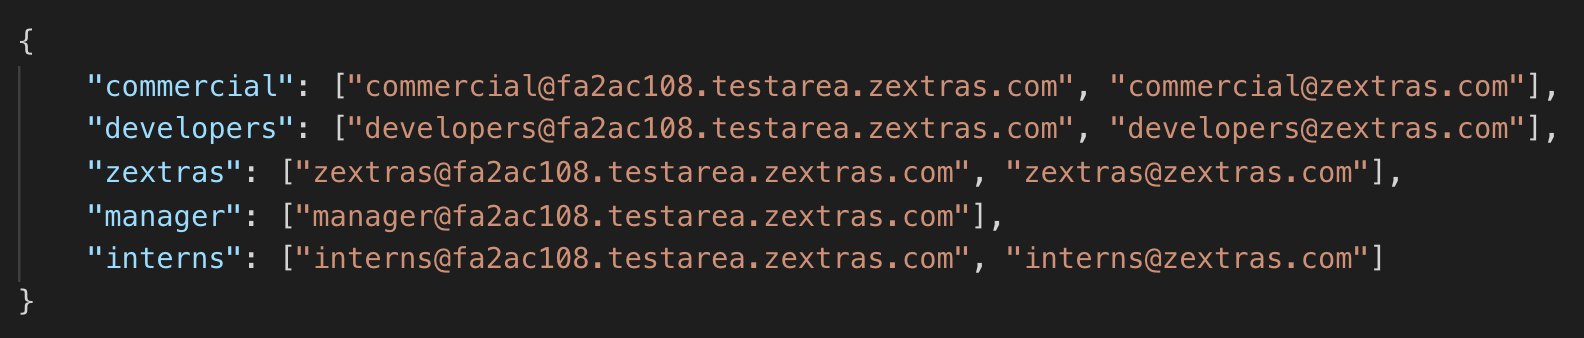
\includegraphics[width=1\textwidth]{immagini/distListMapping.png}
        \caption{Mappatura liste di distribuzione}
        %\textbf{Fonte}:
        %\href{https://www.oasis-open.org/committees/download.php/27819/sstc-saml-tech-overview-2.0-cd-02.pdf}{oasis-open.org}
        \label{fig: Mappatura liste di distribuzione}
    \end{figure}

\subsection{Configurazione Zimbra}
La configurazione di tutto il sistema di autenticazione è stata fatta attraverso la configurazione di \gls{zcsg}, la quale offre la possibilità di definire attributi di diversi tipi, tra cui valori binari (vero o falso), stringhe e oggetti \gls{jsong}. Le mappature descritte nella sezione precedente e illustrate nelle figure \secref{fig: Mappatura classe di servizio} e \secref{fig: Mappatura liste di distribuzione} erano configurate attraverso due attributi specifici. Oltre a questi ne sono stati definiti altri, tra cui:
\begin{itemize}
    \item Configurazione del protocollo \gls{samlg};
    \item Attivazione e disattivazione della creazione automatica di un nuovo \textit{account}  su \gls{zcsg};
    \item Attivazione e disattivazione della sincronizzazione, ad ogni accesso tramite \textit{SAML}, dei gruppi \gls{okta} a cui appartiene un utente con \gls{cosg} e \gls{distlistg}.
\end{itemize}
Questi attributi vengono letti dall'\textit{handler} ogni volta che il sistema di autenticazione riceve una richiesta.

\section{Sviluppo}
Alcuni dettagli di rilievo per quanto riguarda la parte implementativa. In particolare ciò che ho dovuto attuare per superare alcuni ostacoli
\subsection{Parsing SAML assertion}
\subsection{Adattamento libreria HTTP}

\section{Documentazione}
La documentazione è stata presente sin dall'inizio dell'attività di stage, rivelandosi materiale utile sia per tutto il \textit{team}, soprattutto per coloro che non hanno lavorato direttamente con me, ma che necessitano di sapere come funzionano alcuni aspetti del prodotto (per esempio i sistemisti devono sapere come effettuare le configurazioni sul \textit{server}. Inoltre è per chi ora dovrà effettuare la manutenzione dato che potrà risalire a tutto il lavoro da me svolto. Infine mi è stata molto di aiuto durante la presentazione dei miei progressi durante gli incontri con il \textit{Project Manager}.
\subsection{Fase di ricerca}
Durante questa fase ho documentato tutti i risultati dei miei studi in un documento  che illustrava tutti i protocolli analizzati, riportando le informazioni tecniche essenziali e discutendone vantaggi e svantaggi per ciascuno di essi. Questo documento è stato poi aggiornato fino al momento in cui ho scelto, insieme al \textit{team}, il protocollo da utilizzare.
\subsection{Codice}
La documentazione del codice è fondamentale per due motivi: spiegare sezioni difficili da comprendere e facilitare la manutenzione a coloro che dovranno farla, soprattutto se verrà fatta da persone diverse dall'autore. Infatti in una \textit{Sprint Retrospective}, in particolare durante la scrittura dello \textit{Starfish Retrospective} (come descritto nella sezione \secref{sec:met_svilpuppo} è emerso che tutto il \textit{team} avrebbe dovuto dedicare più tempo alla documentazione del codice, scrivendola secondo le regole del \gls{javadocg}.
\subsection{Manutenzione}
Per quanto riguarda la documentazione dell'architettura e della configurazione del prodotto, ho utilizzato \textbf{\textit{Confluence}}, come descritto nella sezione \secref{sec:doc}. Il documento, accessibile a tutti i reparti dell'azienda, era necessario ai sistemisti per poter installare e opportunamente configurare il sistema e al \textit{team}, nel caso in futuro dovesse estenderlo o apportare delle correzioni.

\section{Verifica e Validazione}
Descrizione dell'attività di verifica svolta e della validazione
\subsection{Verifica}
% code review descrizione e immagine
% Mockito e Guice
\subsection{Validazione}
% parlare degli incontri formali e dell'ultimo incontro